%! Author = loreb
%! Date = 31/10/2023

% Preamble
\documentclass[11pt]{article}

% Packages
\usepackage{amsmath}
\usepackage{graphicx}
\usepackage{float}
\usepackage{csvsimple}
\usepackage{hyperref}
\usepackage{listings}
\usepackage{xcolor}
\usepackage{subcaption}
\usepackage{mdwtab}

\definecolor{codegreen}{rgb}{0,0.6,0}
\definecolor{codegray}{rgb}{0.5,0.5,0.5}
\definecolor{codepurple}{rgb}{0.58,0,0.82}
\definecolor{backcolour}{rgb}{0.95,0.95,0.92}

\lstdefinestyle{mystyle}{
    backgroundcolor=\color{backcolour},
    commentstyle=\color{codegreen},
    keywordstyle=\color{magenta},
    numberstyle=\tiny\color{codegray},
    stringstyle=\color{codepurple},
    basicstyle=\ttfamily\footnotesize,
    breakatwhitespace=false,
    breaklines=true,
    captionpos=b,
    keepspaces=true,
    numbers=left,
    numbersep=5pt,
    showspaces=false,
    showstringspaces=false,
    showtabs=false,
    tabsize=2
}
\lstset{style=mystyle}
\graphicspath{{../results/csv/}}

\title{BloomFilter Speedup on setup and filter with Joblib}
\title{%
  Parallelizzazione di un BloomFilter per la classificazione di email di spam \\
  \large Parallel Programming for Machine Learning}
\author{Lorenzo Baiardi, Thomas Del Moro}
\date{GG MM AAAA}

% Document
\begin{document}

    \maketitle
    \clearpage

    \section{Introduzione}\label{sec:introduzione}
    Il nostro progetto si concentra sulla parallelizzazione di un BloomFilter impiegato per la classificazione di email considerate spam.
    Per raggiungere questo obiettivo, utilizziamo le librerie Omp e Joblib per implementare il parallelismo.

    Le fasi che intendiamo parallelizzare sono il setup iniziale e la fase di filtraggio.
    Vogliamo analizzare come lo speedup varia in relazione alle dimensioni dell'insieme di dati utilizzato per il training.
    Allo stesso modo, intendiamo valutare l'effetto dello speedup in funzione del numero di processori impiegati, delle dimensioni del dataset
    e delle diverse implementazioni utilizzate.

    \section{Analisi del problema}\label{sec:analisi-del-problema}
    Il BloomFilter rappresenta una struttura dati probabilistica finalizzata a determinare la presenza di un elemento all'interno di un insieme,
    nel contesto specifico, se una determinata email è considerata spam o meno.
    La fase iniziale di configurazione del BloomFilter coinvolge il calcolo delle funzioni hash e la creazione del vettore di bit.
    Quest'ultima operazione si basa sulla dimensione dell'insieme utilizzato per il training e sulla probabilità attesa di ottenere falsi positivi.
    La formula per il calcolo della dimensione del vettore di bit è la seguente:
    \begin{equation}
        size = -\frac{n \ln{p}}{(\ln{2})^2}\label{eq:dim_bit}
    \end{equation}
    Dove $size$ è la dimensione del vettore di bit per il training e $n$ è la dimensione dell'insieme che si vuole utilizzare.

    La formula per il calcolo del numero di funzioni hash è la seguente:
    \begin{equation}
        h = \frac{size}{n} \ln{2}\label{eq:num_hash}
    \end{equation}
    Dove $h$ è il numero di funzioni hash da utilizzare per il training.

    Dopo aver fornito al BloomFilter il dataset di training, quest'ultimo procede al calcolo delle $h$ funzioni hash per ciascuna email,
    impostando a 1 i bit nelle posizioni calcolate.
    Per determinare se un'email è classificata come spam o meno, il BloomFilter esegue nuovamente il calcolo delle $h$
    funzioni hash e verifica se i bit corrispondenti alle posizioni calcolate sono settati a 1.

    \section{Parallelizzazione}\label{sec:parallelizazzione}
    Il codice sequenziale di riferimento da parallelizzare per la fase di setup è il seguente:
    \lstinputlisting[language=python, firstline=33, lastline=39,label={lst:sequential-code-setup-joblib}]{../src/bloom_filter.py}
    \lstinputlisting[language=c++, firstline=22, lastline=28,label={lst:sequential-code-setup-omp}]{BloomFilter.cpp}

    Il codice sequenziale di riferimento da parallelizzare per la fase di filter è il seguente:
    \lstinputlisting[language=python, firstline=58, lastline=66,label={lst:sequential-code-filter-joblib}]{../src/bloom_filter.py}
    \lstinputlisting[language=c++, firstline=45, lastline=51,label={lst:sequential-code-filter-omp}]{BloomFilter.cpp}

    \subsection{OpenMP (Omp)}\label{subsec:omp}
    OpenMP (Omp) è una libreria in linguaggio C progettata per consentire la parallelizzazione di funzioni e cicli for.
    La funzione \texttt{omp parallel} richiede come input il numero di processori da impiegare e la funzione da parallelizzare.
    Nel contesto di questo lavoro, abbiamo adottato la funzione \texttt{omp parallel for} per parallelizzare le operazioni
    di setup e filtraggio del BloomFilter.

    Successivamente, abbiamo analizzato il tempo impiegato dalle funzioni di setup e filtraggio in relazione al numero
    di processori utilizzati, confrontandolo con il tempo richiesto nella versione sequenziale.
    \lstinputlisting[language=c++, firstline=30, lastline=37, label={lst:sequential-code}]{BloomFilter.cpp}

    \subsection{Joblib}\label{subsec:joblib}
    Joblib è una libreria Python che permette di parallelizzare funzioni e cicli for.
    La funzione Parallel prende in input il numero di processori da utilizzare e la funzione da parallelizzare.
    In questo elaborato abbiamo utilizzato la funzione Parallel per parallelizzare la funzione setup e la funzione
    filter del bloom filter.
    Abbiamo poi successivamente elaborato quanto tempo impiegano le funzioni setup e filter a seconda del numero di
    processori utilizzati rispetto al tempo impiegato nella sua versione sequenziale.
    \lstinputlisting[language=python, firstline=41, lastline=50,label={lst:joblib-code-setup}]{../src/bloom_filter.py}
    \lstinputlisting[language=python, firstline=68, lastline=80,label={lst:joblib-code-filter}]{../src/bloom_filter.py}

    \section{Caratteristiche della macchina}\label{sec:caratteristiche-della-macchina}
    La macchina utilizzata per i test ha le seguenti caratteristiche:
    \begin{itemize}
        \item \textbf{CPU}: Intel Core i7-1360P (4 P-Core, 8 E-Core, 12 Cores, 16 Threads)
        \item \textbf{RAM}: 16GB
        \item \textbf{Sistema Operativo}: Windows 11
    \end{itemize}

    \section{Tests}\label{sec:tests}
    I test sono stati effettuati su un dataset da 1000 fino a 10000000 email, con una probabilità di falsi positivi che
    varia da 0.10 a 0.01.

    \section{Risultati}\label{sec:risultati}
    \subsection{FPR: 0.10}\label{subsec:fpr-010}
    \subsubsection{Setup}\label{subsubsec:fpr-010-setup}
    \begin{figure}[H]
        \centering
        \minipage{0.49\textwidth}
        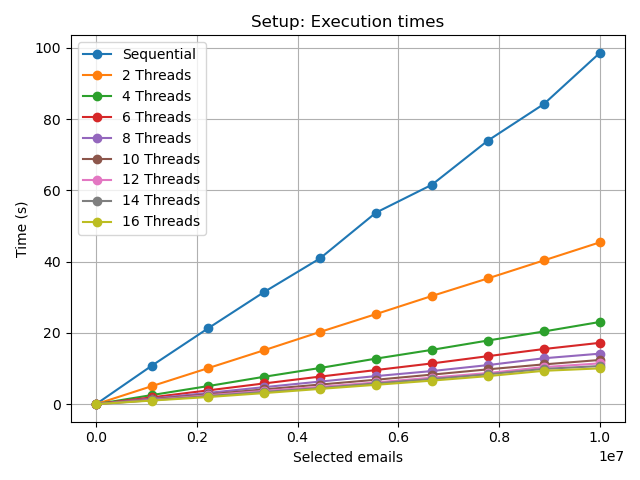
\includegraphics[width=\linewidth]{openmp/010/setup_times}
            \caption{Speedup setup Omp}\label{fig:010-setup_time_omp}
        \endminipage\hfill
        \minipage{0.49\textwidth}
        \includegraphics[width=\linewidth]{/joblib/010/setup_time_plot}
            \caption{Speedup setup Joblib}\label{fig:010setup_time_joblib}
        \endminipage\hfill
        \caption{Time setup}
    \end{figure}
    \begin{figure}[H]
        \centering
        \minipage{0.49\textwidth}
        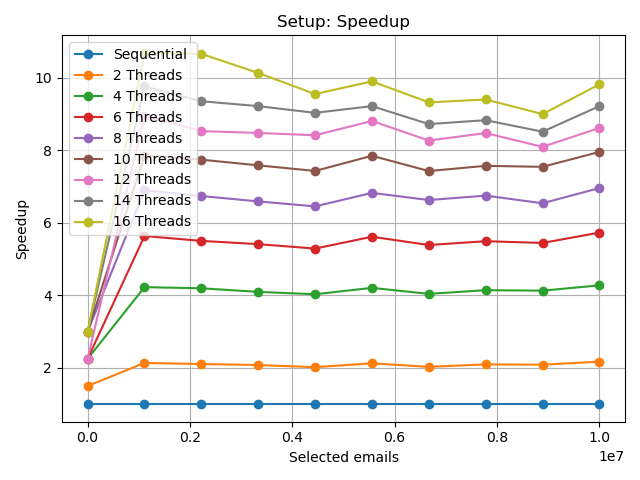
\includegraphics[width=\linewidth]{openmp/010/setup_speedup}
            \caption{Speedup setup Omp}\label{fig:010-setup_speedup_omp}
        \endminipage\hfill
        \minipage{0.49\textwidth}
        \includegraphics[width=\linewidth]{/C:/Users/loreb/Documents/IntellijProjects/PycharmProjects/bloomfilter_parallel/results/csv/joblib/010/setup_speedup_plot}
            \caption{Speedup setup Joblib}\label{fig:010-setup_speedup_joblib}
        \endminipage\hfill
        \caption{Speedup setup}
    \end{figure}
    \begin{figure}[H]
        \centering
        \minipage{0.49\textwidth}
        \includegraphics[width=\linewidth]{omp/010/setup_fpr_plot}
            \caption{Speedup setup Omp}\label{fig:010-setup_fpr_omp}
        \endminipage\hfill
        \minipage{0.49\textwidth}
        \includegraphics[width=\linewidth]{/C:/Users/loreb/Documents/IntellijProjects/PycharmProjects/bloomfilter_parallel/results/csv/joblib/010/setup_fpr_plot}
            \caption{Speedup setup Joblib}\label{fig:010-setup_fpr_joblib}
        \endminipage\hfill
        \caption{Time setup}
    \end{figure}
    \subsubsection{Filter}\label{subsubsec:fpr-010-filter}
    \begin{figure}[H]
        \centering
        \minipage{0.49\textwidth}
        \includegraphics[width=\linewidth]{omp/010/filter_time_plot}
            \caption{Speedup setup Omp}\label{fig:010-filter_time_omp}
        \endminipage\hfill
        \minipage{0.49\textwidth}
        \includegraphics[width=\linewidth]{/C:/Users/loreb/Documents/IntellijProjects/PycharmProjects/bloomfilter_parallel/results/csv/joblib/010/filter_time_plot}
            \caption{Speedup setup Joblib}\label{fig:010-filter_time_joblib}
        \endminipage\hfill
        \caption{Time setup}
    \end{figure}
    \begin{figure}[H]
        \centering
        \minipage{0.49\textwidth}
        \includegraphics[width=\linewidth]{omp/010/filter_speedup_plot}
            \caption{Speedup setup Omp}\label{fig:010-filter_speedup_omp}
        \endminipage\hfill
        \minipage{0.49\textwidth}
        \includegraphics[width=\linewidth]{/C:/Users/loreb/Documents/IntellijProjects/PycharmProjects/bloomfilter_parallel/results/csv/joblib/010/filter_speedup_plot}
            \caption{Speedup setup Joblib}\label{fig:010-filter_speedup_joblib}
        \endminipage\hfill
        \caption{Speedup setup}
    \end{figure}
    \begin{figure}[H]
        \centering
        \minipage{0.49\textwidth}
        \includegraphics[width=\linewidth]{omp/010/filter_fpr_plot}
            \caption{Speedup setup Omp}\label{fig:010-filter_fpr_omp}
        \endminipage\hfill
        \minipage{0.49\textwidth}
        \includegraphics[width=\linewidth]{/C:/Users/loreb/Documents/IntellijProjects/PycharmProjects/bloomfilter_parallel/results/csv/joblib/010/filter_fpr_plot}
            \caption{Speedup setup Joblib}\label{fig:010-filter_fpr_joblib}
        \endminipage\hfill
        \caption{Time setup}
    \end{figure}
    \subsubsection{Chunks}\label{subsubsec:010-chunks}
    \begin{figure}[H]
        \centering
        \minipage{0.49\textwidth}
        \includegraphics[width=\linewidth]{/C:/Users/loreb/Documents/IntellijProjects/PycharmProjects/bloomfilter_parallel/results/csv/joblib/010/chunks_time_plot}
            \caption{Times setup Chunk}\label{fig:010-chunks_time}
        \endminipage\hfill
        \minipage{0.49\textwidth}
        \includegraphics[width=\linewidth]{/C:/Users/loreb/Documents/IntellijProjects/PycharmProjects/bloomfilter_parallel/results/csv/joblib/010/chunks_speedup_plot}
            \caption{Speedup setup Chunk}\label{fig:010-chunks_speedup}
        \endminipage\hfill
        \caption{Time setup}
    \end{figure}

    \subsection{FPR: 0.05}\label{subsec:fpr-005}
    \subsubsection{Setup}\label{subsubsec:fpr-005-setup}
    \begin{figure}[H]
        \centering
        \minipage{0.49\textwidth}
        \includegraphics[width=\linewidth]{omp/005/setup_time_plot}
            \caption{Speedup setup Omp}\label{fig:005-setup_time_omp}
        \endminipage\hfill
        \minipage{0.49\textwidth}
        \includegraphics[width=\linewidth]{/C:/Users/loreb/Documents/IntellijProjects/PycharmProjects/bloomfilter_parallel/results/csv/joblib/005/setup_time_plot}
            \caption{Speedup setup Joblib}\label{fig:005-setup_time_joblib}
        \endminipage\hfill
        \caption{Time setup}
    \end{figure}
    \begin{figure}[H]
        \centering
        \minipage{0.49\textwidth}
        \includegraphics[width=\linewidth]{omp/005/setup_speedup_plot}
            \caption{Speedup setup Omp}\label{fig:005-setup_speedup_omp}
        \endminipage\hfill
        \minipage{0.49\textwidth}
        \includegraphics[width=\linewidth]{/C:/Users/loreb/Documents/IntellijProjects/PycharmProjects/bloomfilter_parallel/results/csv/joblib/005/setup_speedup_plot}
            \caption{Speedup setup Joblib}\label{fig:005-setup_speedup_joblib}
        \endminipage\hfill
        \caption{Speedup setup}
    \end{figure}
    \begin{figure}[H]
        \centering
        \minipage{0.49\textwidth}
        \includegraphics[width=\linewidth]{omp/005/setup_fpr_plot}
            \caption{Speedup setup Omp}\label{fig:005-setup_fpr_omp}
        \endminipage\hfill
        \minipage{0.49\textwidth}
        \includegraphics[width=\linewidth]{/C:/Users/loreb/Documents/IntellijProjects/PycharmProjects/bloomfilter_parallel/results/csv/joblib/005/setup_fpr_plot}
            \caption{Speedup setup Joblib}\label{fig:005-setup_fpr_joblib}
        \endminipage\hfill
        \caption{Time setup}
    \end{figure}
    \subsubsection{Filter}\label{subsubsec:fpr-005-filter}
    \begin{figure}[H]
        \centering
        \minipage{0.49\textwidth}
        \includegraphics[width=\linewidth]{omp/005/filter_time_plot}
            \caption{Speedup setup Omp}\label{fig:005-filter_time_omp}
        \endminipage\hfill
        \minipage{0.49\textwidth}
        \includegraphics[width=\linewidth]{/C:/Users/loreb/Documents/IntellijProjects/PycharmProjects/bloomfilter_parallel/results/csv/joblib/005/filter_time_plot}
            \caption{Speedup setup Joblib}\label{fig:005-filter_time_joblib}
        \endminipage\hfill
        \caption{Time setup}
    \end{figure}
    \begin{figure}[H]
        \centering
        \minipage{0.49\textwidth}
        \includegraphics[width=\linewidth]{omp/005/filter_speedup_plot}
            \caption{Speedup setup Omp}\label{fig:005-filter_speedup_omp}
        \endminipage\hfill
        \minipage{0.49\textwidth}
        \includegraphics[width=\linewidth]{/C:/Users/loreb/Documents/IntellijProjects/PycharmProjects/bloomfilter_parallel/results/csv/joblib/005/filter_speedup_plot}
            \caption{Speedup setup Joblib}\label{fig:005-filter_speedup_joblib}
        \endminipage\hfill
        \caption{Speedup setup}
    \end{figure}
    \begin{figure}[H]
        \centering
        \minipage{0.49\textwidth}
        \includegraphics[width=\linewidth]{omp/005/filter_fpr_plot}
            \caption{Speedup setup Omp}\label{fig:005-filter_fpr_omp}
        \endminipage\hfill
        \minipage{0.49\textwidth}
        \includegraphics[width=\linewidth]{/C:/Users/loreb/Documents/IntellijProjects/PycharmProjects/bloomfilter_parallel/results/csv/joblib/005/filter_fpr_plot}
            \caption{Speedup setup Joblib}\label{fig:005-filter_fpr_joblib}
        \endminipage\hfill
        \caption{Time setup}
    \end{figure}
    \subsubsection{Chunks}\label{subsubsec:005-chunks}
    \begin{figure}[H]
        \centering
        \minipage{0.49\textwidth}
        \includegraphics[width=\linewidth]{/C:/Users/loreb/Documents/IntellijProjects/PycharmProjects/bloomfilter_parallel/results/csv/joblib/005/chunks_time_plot}
            \caption{TImes setup Chunks}\label{fig:005-chunks_time}
        \endminipage\hfill
        \minipage{0.49\textwidth}
        \includegraphics[width=\linewidth]{/C:/Users/loreb/Documents/IntellijProjects/PycharmProjects/bloomfilter_parallel/results/csv/joblib/005/chunks_speedup_plot}
            \caption{Speedup setup Chunks}\label{fig:005-chunks_speedup}
        \endminipage\hfill
        \caption{Time setup}
    \end{figure}

    \subsection{FPR: 0.01}\label{subsec:fpr-001}
    \subsubsection{Setup}\label{subsubsec:setup}
    \begin{figure}[H]
        \centering
        \minipage{0.49\textwidth}
        \includegraphics[width=\linewidth]{omp/001/setup_time_plot}
            \caption{Speedup setup Omp}\label{fig:setup_time_omp}
        \endminipage\hfill
        \minipage{0.49\textwidth}
        \includegraphics[width=\linewidth]{/C:/Users/loreb/Documents/IntellijProjects/PycharmProjects/bloomfilter_parallel/results/csv/joblib/001/setup_time_plot}
            \caption{Speedup setup Joblib}\label{fig:setup_time_joblib}
        \endminipage\hfill
        \caption{Time setup}
    \end{figure}
    \begin{figure}[H]
        \centering
        \minipage{0.49\textwidth}
        \includegraphics[width=\linewidth]{omp/001/setup_speedup_plot}
            \caption{Speedup setup Omp}\label{fig:setup_speedup_omp}
        \endminipage\hfill
        \minipage{0.49\textwidth}
        \includegraphics[width=\linewidth]{/C:/Users/loreb/Documents/IntellijProjects/PycharmProjects/bloomfilter_parallel/results/csv/joblib/001/setup_speedup_plot}
            \caption{Speedup setup Joblib}\label{fig:setup_speedup_joblib}
        \endminipage\hfill
        \caption{Speedup setup}
    \end{figure}
    \begin{figure}[H]
        \centering
        \minipage{0.49\textwidth}
        \includegraphics[width=\linewidth]{omp/001/setup_fpr_plot}
            \caption{Speedup setup Omp}\label{fig:setup_fpr_omp}
        \endminipage\hfill
        \minipage{0.49\textwidth}
        \includegraphics[width=\linewidth]{/C:/Users/loreb/Documents/IntellijProjects/PycharmProjects/bloomfilter_parallel/results/csv/joblib/001/setup_fpr_plot}
            \caption{Speedup setup Joblib}\label{fig:setup_fpr_joblib}
        \endminipage\hfill
        \caption{Time setup}
    \end{figure}

    \subsubsection{Filter}\label{subsubsec:filter}
    \begin{figure}[H]
        \centering
        \minipage{0.49\textwidth}
        \includegraphics[width=\linewidth]{omp/001/filter_time_plot}
            \caption{Times filter Omp}\label{fig:filter_time_omp}
        \endminipage\hfill
        \minipage{0.49\textwidth}
        \includegraphics[width=\linewidth]{/C:/Users/loreb/Documents/IntellijProjects/PycharmProjects/bloomfilter_parallel/results/csv/joblib/001/filter_time_plot}
            \caption{Times filter Joblib}\label{fig:filter_time_joblib}
        \endminipage\hfill
        \caption{Time filter}
    \end{figure}
    \begin{figure}[H]
        \centering
        \minipage{0.49\textwidth}
        \includegraphics[width=\linewidth]{omp/001/filter_speedup_plot}
            \caption{Speedup filter Omp}\label{fig:filter_speedup_omp}
        \endminipage\hfill
        \minipage{0.49\textwidth}
        \includegraphics[width=\linewidth]{/C:/Users/loreb/Documents/IntellijProjects/PycharmProjects/bloomfilter_parallel/results/csv/joblib/001/filter_speedup_plot}
            \caption{Speedup filter Joblib}\label{fig:filter_speedup_joblib}
        \endminipage\hfill
        \caption{Speedup filter}
    \end{figure}
    \begin{figure}[H]
        \centering
        \minipage{0.49\textwidth}
        \includegraphics[width=\linewidth]{omp/001/filter_fpr_plot}
            \caption{FPR filter Omp}\label{fig:filter_fpr_omp}
        \endminipage\hfill
        \minipage{0.49\textwidth}
        \includegraphics[width=\linewidth]{/C:/Users/loreb/Documents/IntellijProjects/PycharmProjects/bloomfilter_parallel/results/csv/joblib/001/filter_fpr_plot}
            \caption{FPR filter Joblib}\label{fig:filter_fpr_joblib}
        \endminipage\hfill
        \caption{Time filter}
    \end{figure}

    \subsubsection{Chunks}\label{subsubsec:chunks}
    \begin{figure}[H]
        \centering
        \minipage{0.49\textwidth}
        \includegraphics[width=\linewidth]{/C:/Users/loreb/Documents/IntellijProjects/PycharmProjects/bloomfilter_parallel/results/csv/joblib/001/chunks_time_plot}
            \caption{Times chunks Joblib}\label{fig:chunks_time_joblib}
        \endminipage\hfill
        \minipage{0.49\textwidth}
        \includegraphics[width=\linewidth]{/C:/Users/loreb/Documents/IntellijProjects/PycharmProjects/bloomfilter_parallel/results/csv/joblib/001/chunks_speedup_plot}
            \caption{Speedup chunks Joblib}\label{fig:chunks_speedup_joblib}
        \endminipage\hfill
        \caption{Speedup chunks}
    \end{figure}

    \section{Conclusioni}\label{sec:conclusioni}
    Dai risultati ottenuti possiamo vedere come il valore di Speedup massimo si attesti intorno a 3 rispetto alla versione sequenziale.
    In generale possiamo notare come lo speedup aumenti con l'aumentare della dimensione dell'insieme, fino a un certo punto per la versione Joblib.

    \clearpage

    \section{Dati}\label{sec:dati}
    \begin{figure}[H]
        \csvautotabular{../results/csv/setup.csv}\label{fig:setup_csv}
    \end{figure}
    \begin{figure}[H]
        \csvautotabular{../results/csv/filter.csv}\label{fig:filter_csv}
    \end{figure}
    \begin{figure}[H]
        \csvautotabular{../results/csv/chunks.csv}\label{fig:chunks_csv}
    \end{figure}


\end{document}